\begin{figure}[tbp]
\centering
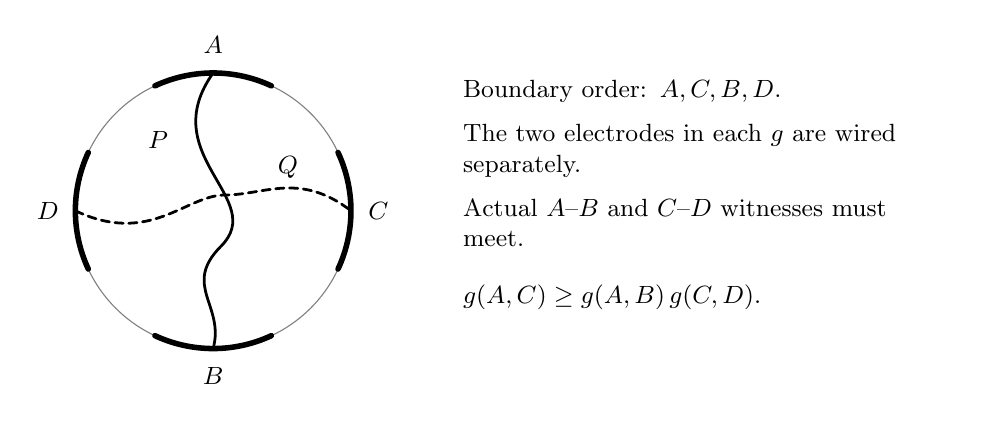
\begin{tikzpicture}[x=1cm,y=1cm,font=\small,line cap=round,line join=round]
  \draw[gray] (0,0) circle (1.75);
  \foreach \start/\finish/\name/\angle in {65/115/A/90,-25/25/C/0,-115/-65/B/-90,155/205/D/180} {
    \draw[line width=2pt] (\start:1.75) arc (\start:\finish:1.75);
    \node at (\angle:2.1) {$\name$};
  }
  \draw[line width=1pt] (0,1.75) .. controls (-.75,.7) and (.7,.15) .. (.1,-.45)
    .. controls (-.4,-.95) and (.15,-1.2) .. (0,-1.75);
  \draw[densely dashed,line width=1pt] (-1.75,0) .. controls (-.8,-.45) and (-.35,.2) .. (.15,.2)
    .. controls (.65,.2) and (1.1,.5) .. (1.75,0);
  \node[fill=white,inner sep=1.5pt] at (-.7,.9) {$P$};
  \node[fill=white,inner sep=1.5pt] at (.95,.55) {$Q$};
  \node[align=left,anchor=west,text width=6.1cm] at (3.05,.6)
    {Boundary order: $A,C,B,D$.\\[5pt]
     The two electrodes in each $g$ are wired separately.\\[5pt]
     Actual $A$--$B$ and $C$--$D$ witnesses must meet.};
  \node[anchor=west] at (3.05,-1.1)
    {$g(A,C)\geq g(A,B)\,g(C,D)$.};
\end{tikzpicture}
\caption{The topology behind interlacing gluing. Thick boundary arcs mark the four electrode sets, not a common four-wire law: each probability $g$ wires only its own two electrodes. The curves $P,Q$ illustrate actual witnesses and their forced meeting, not simultaneous events under one boundary condition. The probability inequality uses the restricted comparison and the extremal exploration in Lemma~\ref{lem:interlacing}, not positive association or independence.}
\label{fig:interlacing}
\end{figure}
